\begin{figure*}
    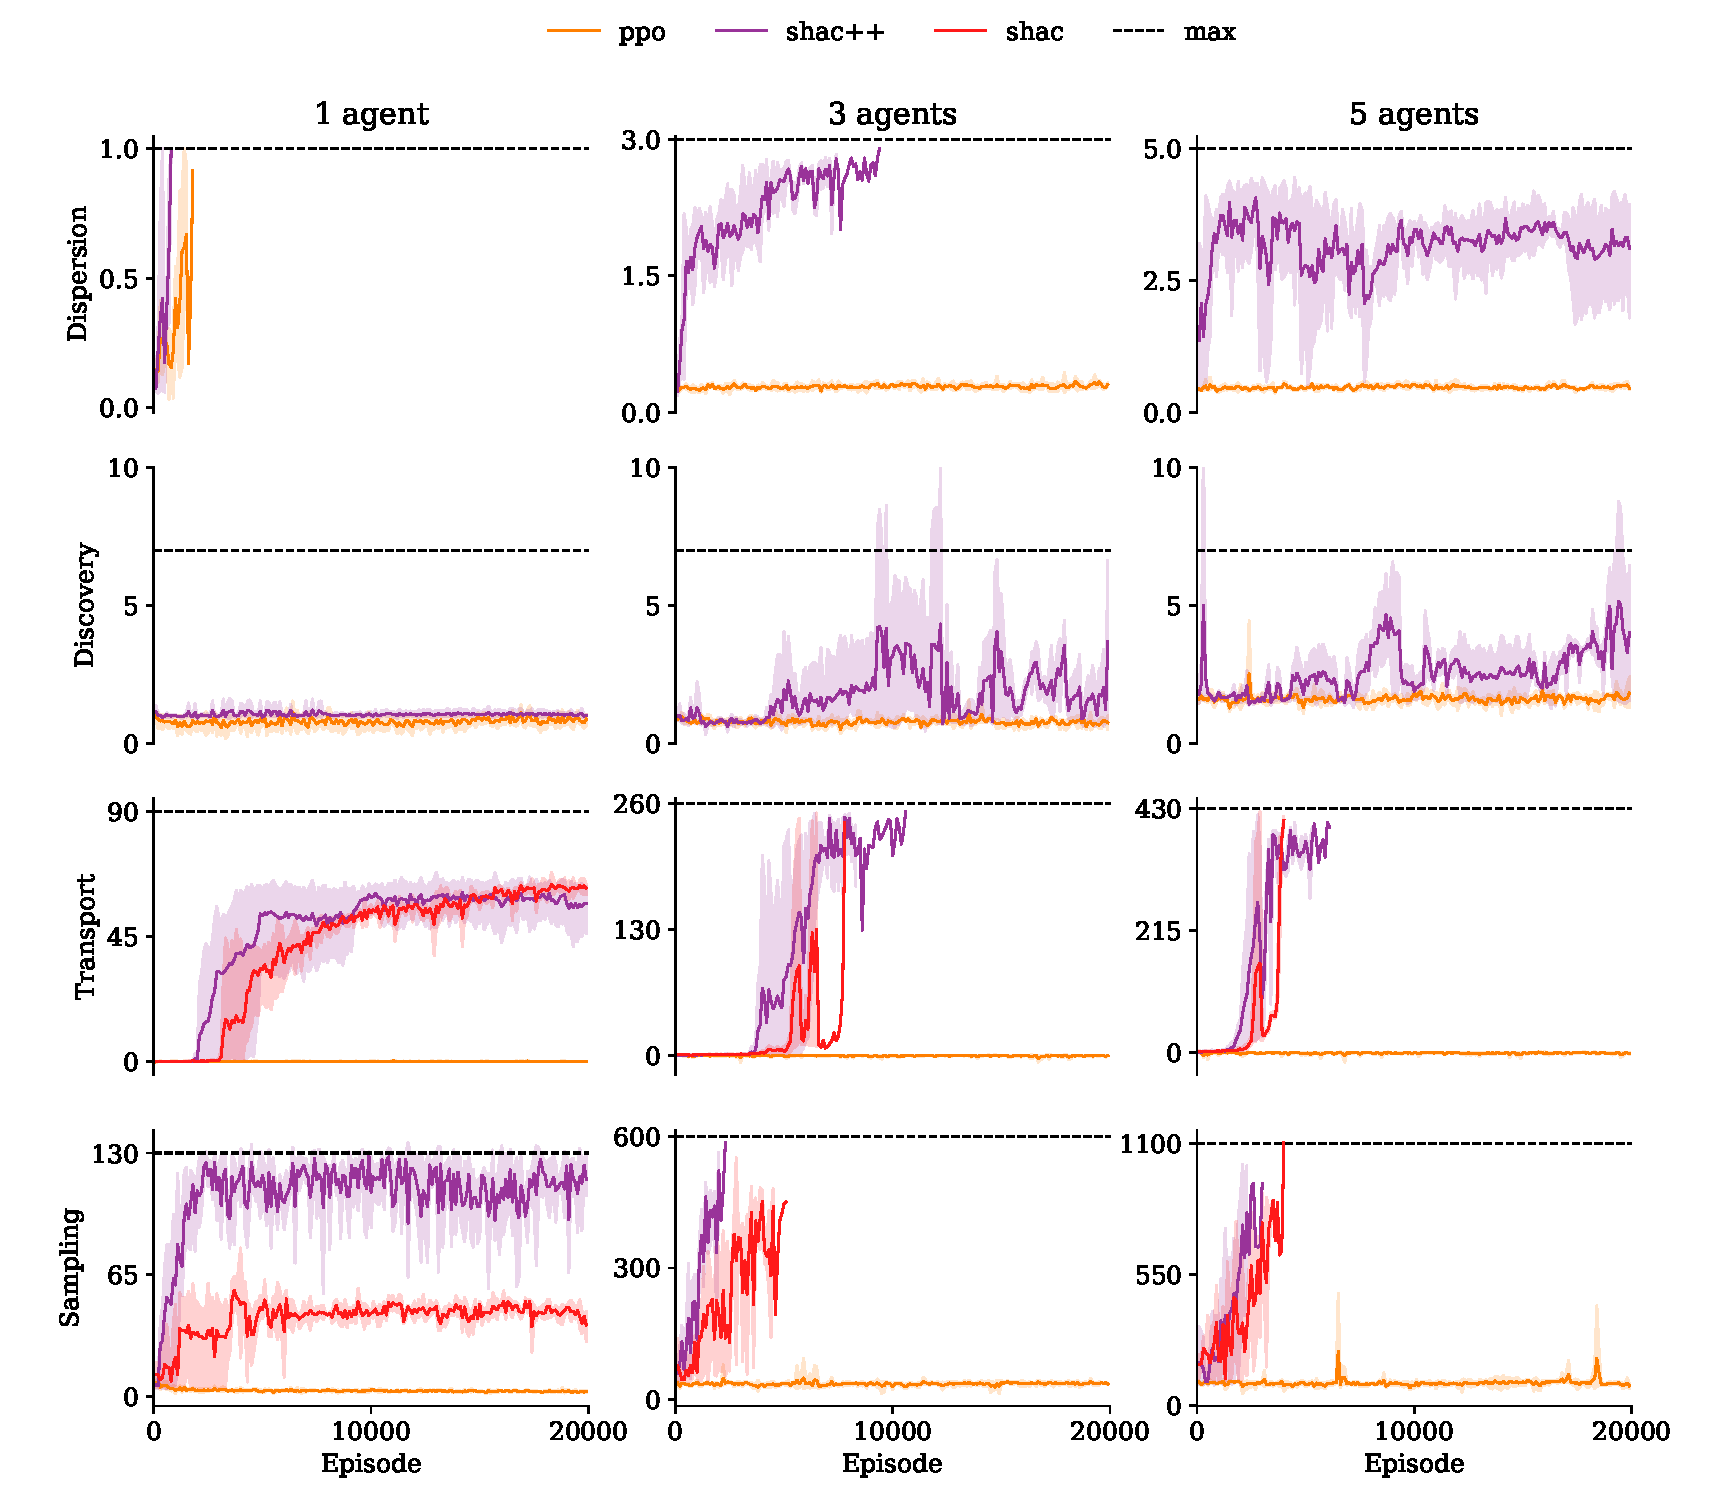
\includegraphics[width=\textwidth]{figs/main-transformer.pdf}
    \caption{Performance comparison of \fname{}, PPO, and SHAC across different scenarios (Dispersion, Transport, Discovery, and Sampling) using the Transformer architecture for multi-agent settings and the MLP architecture for single-agent settings. The results show the mean and standard deviation of rewards over 3 runs. For results using the MLP architecture in all scenarios, refer to \Cref{apx:fig:experiments-mlp}.}%
    \label{fig:experiments}
\end{figure*}

\begin{figure}
    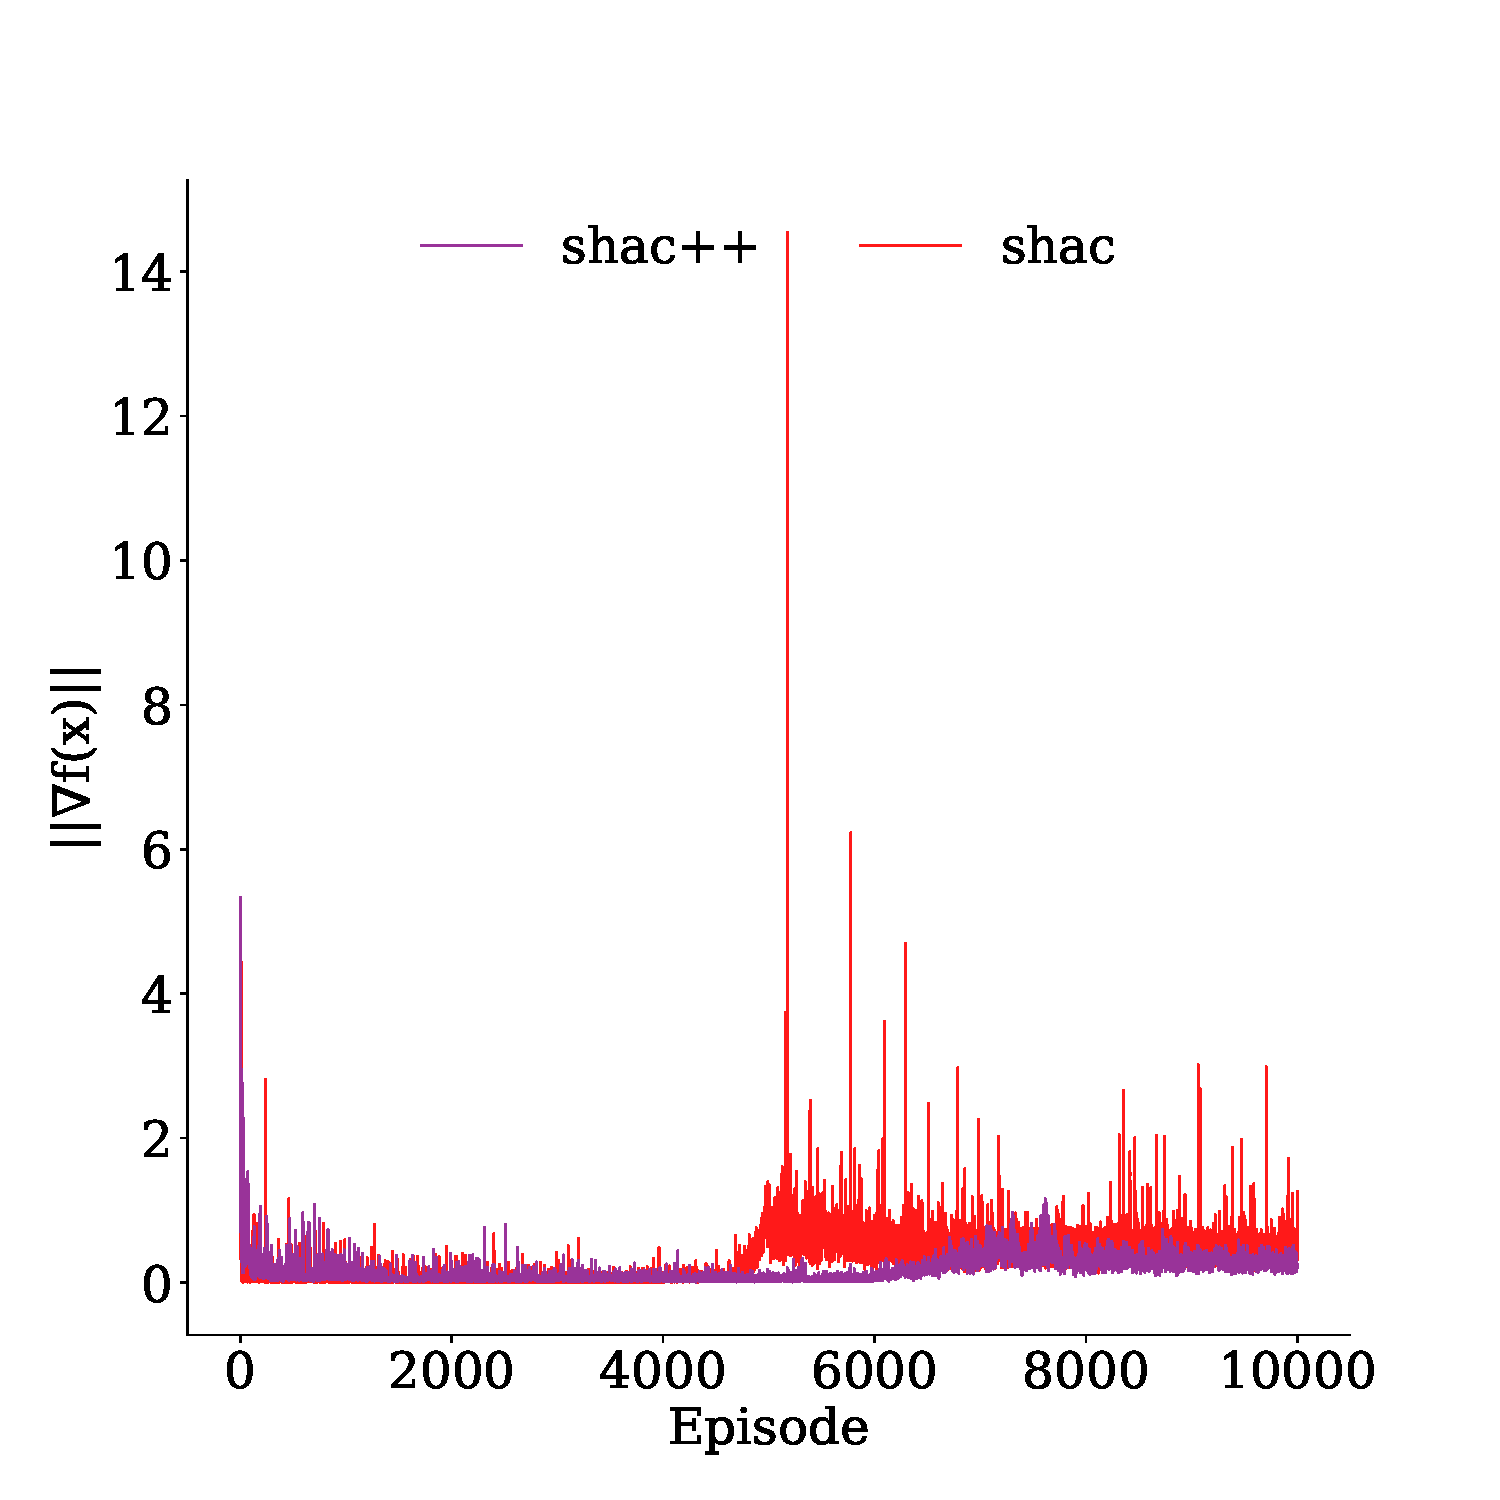
\includegraphics[width=\columnwidth]{figs/grads-transformer-transport.pdf}
    \caption{Norm of policy gradients on the Transport environment across 5000 epochs. The raise in norm for SHAC (epoch 2700) corresponds with occurrence of generalization, where collision between agents and the packages become frequent. Also \fname{} experience a raise in norm, albeit more behaved, corresponds with the occurrence of generalization (epoch 3200).}\label{fig:grads-transformer-transport}

\end{figure}

\section{Experiments}\label{sect:experiments}

In this section, we test \fname{} with PPO and SHAC for a set of multi-agent scenarios and architectures. An ablation study when replacing only the transition function (meaning that the reward function is assumed differentiable) is also conducted in \Cref{apx:ablation}.

\paragraph{Scenarios}
As mentioned previously, we choose a few multi-agent scenarios from the VMAS package to test \fname{}, SHAC and PPO\@. In particular, we choose the scenarios Dispersion, Discovery, Transport, and Sampling. For details regarding each scenario, see \Cref{apx:scenarios}. Dispersion and Discovery have non-differentiable reward functions, thus SHAC is not applicable. Transport and Sampling have differentiable reward functions, thus SHAC is applicable. For Transport and Dispersion, the observation space is complete wrt.\ the state. For Discovery and Sampling, the observation space is incomplete wrt.\ the state. In these scenario, \fname{} is slightly disadvantaged as it does not have access to the full state of the environment compared to SHAC\@.

\begin{table*}[t]
    \centering
    \input tables/max.tex
    \caption{Normalized rewards (relative to the best performing model) for the different scenarios. Best results are in bold.}\label{tab:max-rewards}
\end{table*}

\paragraph{Architectures}
We test SHAC, PPO, and \fname{} with both an MLP and a Transformer architecture. Specifically, we use a 1-layer MLP or a 1-layer single-head Transformer for policy, reward, and value network. The transition network used by \fname{} is always a 3-layer single-head Transformer

While the MLP architecture is the simplest, the Transformer baseline benefits from positional invariance property of the agents observations. We apply the transformer architecture only if the number of agents is greater than $1$, otherwise we use only the MLP architecture. For more details on the architectures, see \Cref{apx:arch}.

\paragraph{Hyperparameters}
For all networks we use learning rate of $1e\text{-}3$ with Adam Optimizer~\cite{Kingma14}. For all scenarios, each training episode consists of $512$ environments of $32$ steps each. Each validation episode is composed of $512$ environments of $512$ steps each. We employ early stopping when the agents achieve $90\%$ of the maximum reward in $90\%$ of the episode's environments. If early stopping is not triggered, we stop training after $20,000$ episodes. The discount factor is set to $0.99$ and lambda factor is set to $0.95$. We report results for increasing number of agents $n\in\{1,3,5\}$. We repeat and report results for $3$ runs with different seeds. See \Cref{apx:tab:ppo} and \Cref{apx:tab:shac} for a complete list of hyperparameters.

Overall, considering different training algorithms, architectures, scenarios, hyperparameters, we completed a total of $254$ runs lasting between $1$ to $8$ hours each. 

\paragraph{Hardware Setup}
Our experiments were conducted on a cluster of machines composed of 2 computational nodes, each with one NVIDIA Tesla V100 GPU (with 32GB of memory), 200GB of RAM, and two Intel Xeon Gold 6226R processors (32 cores each).

\subsection{Results}
In this section, we compare the performance of \fname{}, PPO, and SHAC across different scenarios using the Transformer architecture for multi-agent settings and the MLP architecture for single-agent settings. The results show the mean and standard deviation of achieved rewards over 3 runs. An overview of the results is shown in \Cref{fig:experiments} and \Cref{tab:max-rewards}. For results using the MLP architecture in all scenarios, refer to \Cref{apx:fig:experiments-mlp}.

\paragraph{Dispersion}
In \Cref{fig:experiments}, the first row displays results for the dispersion scenario (non-differentiable, thus SHAC is not applicable). In the first column (single agent, see also \Cref{tab:max-rewards} and \Cref{apx:fig:experiments-mlp}), both PPO and \fname{} perform well, though \fname{} converges faster thanks to gradient approximation. In the second column (3 agents), PPO fails to converge, whereas \fname{} converges in fewer than 10,000 episodes, suggesting emergent cooperative behavior. In the third column (5 agents), PPO fails to converge, while \fname{} achieves high rewards (with no early stopping) but shows high variance due to increased environment complexity.

\paragraph{Discovery} 
The second row of \Cref{fig:experiments} shows a scenario with partial observability, namely discovery. In the first column (single agent), \fname{} outperforms PPO, though it does not reach the maximum reward, suggesting the world model struggles to capture dynamics. In the second and third columns (3 and 5 agents), PPO again fails to converge, whereas \fname{} maintains superior results, indicating cooperative behavior.

\paragraph{Transport}
The third row of \Cref{fig:experiments} presents a differentiable scenario, transport. In the first column (single agent), PPO fails to converge, while SHAC and \fname{} achieve comparable performance.\ \fname{} converges faster, but SHAC is more consistent. In the second and third columns (3 and 5 agents), PPO fails as in the single-agent case, while SHAC and \fname{} both complete the task around 10,000 episodes. With more agents, convergence is faster because the task becomes easier (as more agents can push the package). The emergent of cooperation can be also display but looking to the gradient norm in \Cref{fig:grads-transformer-transport} we can see that the norm of the gradients for SHAC and \fname{} increases when the agents start to collide with each other and the package. This is a sign of generalization, as the agents learn to avoid collisions and push the package together.

\paragraph{Sampling}
The fourth row of \Cref{fig:experiments} illustrates the sampling scenario, which is differentiable and thus applicable to SHAC\@. In the first column (single agent), PPO fails to converge, while \fname{} outperforms SHAC\@. In the second and third columns (3 and 5 agents), PPO again fails to converge, while SHAC and \fname{} both complete training in fewer than 5,000 episodes. Notably, SHAC does not exhibit the same stability advantage it displayed in other scenarios, possibly because gradients derived directly from the environment are noisier compared to those learned by the transition network.
